\chapter{Intrinsic Computation of Centroidal Voronoi Tessellation (CVT) on Meshes}

\section{Introduction}
\label{sec:introduction}

\begin{figure}[htbp]
\centering
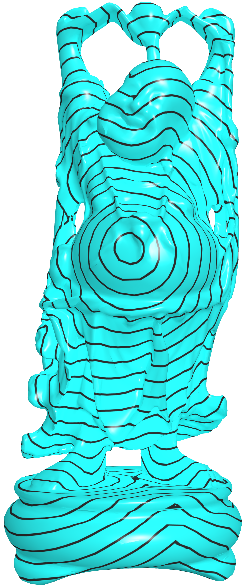
\includegraphics[width=0.3\textwidth]{figs/svg/buddha_nf40k_svg_RMS_0_16.png}
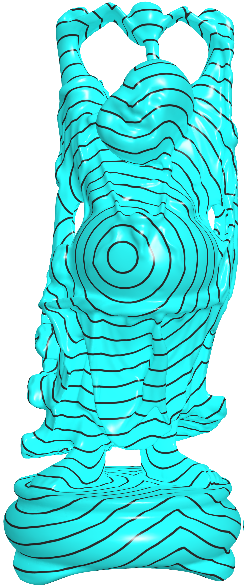
\includegraphics[width=0.3\textwidth]{figs/svg/buddha_nf300k_svg_RMS_0_11.png}
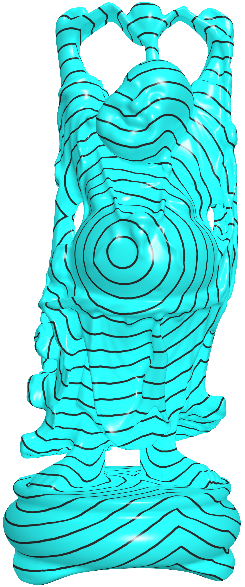
\includegraphics[width=0.3\textwidth]{figs/svg/buddha_nf600k_SVG_RMS_0_12.png}\\
 { \setlength{\fboxsep}{0pt} \setlength{\fboxrule}{1pt}\fbox{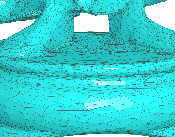
\includegraphics[width=0.3\textwidth]{figs/svg/buddha_nf40k_base_closeup.png}}}
 {   \setlength{\fboxsep}{0pt} \setlength{\fboxrule}{1pt}\fbox{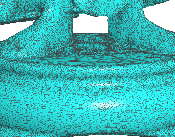
\includegraphics[width=0.3\textwidth]{figs/svg/buddha_nf300k_base_closeup.png}}}
 {   \setlength{\fboxsep}{0pt}
 \setlength{\fboxrule}{1pt}\fbox{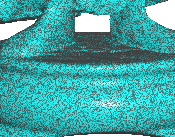
\includegraphics[width=0.3\textwidth]{figs/svg/buddha_nf600k_base_closeup.png}}}\\
\begin{scriptsize}
\makebox[0.3\textwidth]{$(0.37\%, 0.15\%, 0.11\%)$} \makebox[0.3\textwidth]{$(0.35\%,0.13\%,0.11\%)$} \makebox[0.3\textwidth]{$(0.29\%,0.13\%,0.11\%)$}\\
\end{scriptsize}
\vspace{-0.1in} \caption{The SVG method is numerically stable and
the approximated geodesic distances are insensitive to the mesh
tessellation and resolution. From left to right: 40K-face, 300K-face
and 600K-face. The same parameter $K=30$ applying to all three cases
produces consistently high quality results. } \label{fig:buddha}
\end{figure} 